\documentclass[10pt]{article}
\usepackage[utf8]{inputenc}
\usepackage[T1]{fontenc}
\usepackage[version=4]{mhchem}
\usepackage{stmaryrd}
\usepackage[margin=0.5in, tmargin=1in]{geometry}
\usepackage{xcolor}
\usepackage{graphicx}

\usepackage{fancyhdr}
\pagestyle{fancy}
\fancyhf{}
\fancyhead[L]{Math 1A Spring 2024 Notes}
\fancyhead[R]{Alexis Fernandez}
\renewcommand{\headrulewidth}{0.4pt}

\usepackage{enumitem}
\setlist[enumerate]{leftmargin=*}

\usepackage{amsmath, amsfonts, amssymb}

\author{}
\date{}


\begin{document}

\section*{\centering Note 1 - Functions \& Domains}

\subsection*{Function Definitions}

\begin{itemize}
    \item \textbf{Function}: A rule or law that governs the relationship between two variables in which the values of one variable depend on the names of the other variable.
    $$y = f(x)$$
    In the above equation, {\color{blue}$x$} is the {\color{blue}independent variable} and {\color{red}$f(x)$} is the {\color{red}dependent variable}.
    \item \textbf{Domain}: The set of all real numbers (inputs), {\color{blue}$x$}, for which the function is defined or exists.
    \item \textbf{Range}: The set of all real numbers (outputs), {\color{red}$f(x)$/$y$}, for which the function is defined or exists.\\
    \textit{Note: The variable names {\color{blue}$x$}, {\color{red}$f(x)$}, and {\color{red}$y$} are standard, but are also arbitrary.}
    \item \textbf{Piecewise function}: A function that is defined by different formulas in different parts of the domain.

    For example, the absolute value function is defined as
    $$ |x| = \begin{cases}
        -x, \text{ if } x < 0 \\
        x, \text{ if } x \geq 0 \\
        \end{cases}$$
    \item \textbf{Even function}: A function that satisfies $f(-x) = f(x)$ for every number $x$ in its domain.\\
    For example, 
    \begin{align*}
    f(-x) &= (-x)^2 \\ &= x^2 \\ &= f(x)
    \end{align*}
    
    \item \textbf{Odd function}: A function that satisfies $f(-x) = -f(x)$ for every number $x$ in its domain. \\
    For example,
    \begin{align*}
    f(-x) &= (-x)^3 \\ &= -x^3 \\ &= -f(x)
    \end{align*}
    \item \textbf{Increasing function}: A function is increasing on an interval if $f(x_1) < f(x_2)$ when $x_1 < x_2$ on the interval.
    \item \textbf{Decreasing function}: A function is decreasing on an interval if $f(x_1) > f(x_2)$ when $x_1 < x_2$ on the interval.
    \item \textbf{Vertical line test}: A curve in the $xy$-plane is the graph of a function of $x$ if and only if no vertical line passes through the curve more than once. \\
    For example, the vertical line test tells us that for $y=x^2$ and $x=y^2$:
    \begin{figure}[h]
        \centering
        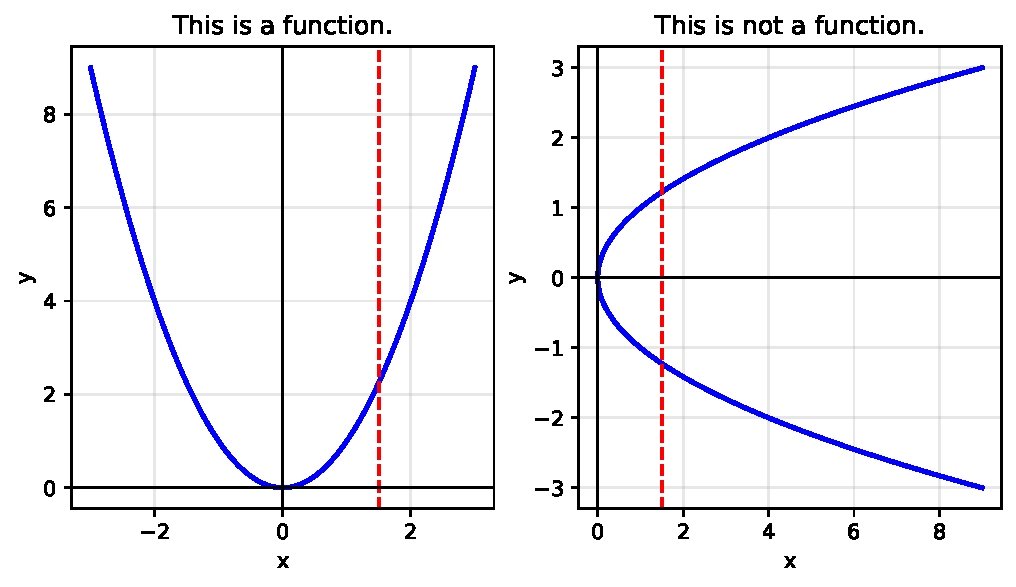
\includegraphics[height=6cm]{images/note01/vlt.pdf}
    \end{figure} 
\end{itemize}


\newpage

\subsection*{Methods for Finding the Domain}

\textbf{Method 1:} Fractional (Rational) Functions\\
{\color{magenta}
\textbf{Procedure:} Find values of $x$ that make the denominator 0.}
\begin{itemize}
    \item Set denominator equal to 0 and solve for $x$.
    \item The domain is the set of all real numbers except the values of x found in previous step. \\
    \textit{Recall: A denominator of 0 makes the function undefined.}
\end{itemize}
{\color{blue}
\textbf{Example:}} $h(x) = \dfrac{3-x}{2x+1}$

    \begin{align*}
    2x+1 &= 0 \qquad \text{\color{magenta}{Set the denominator equal to 0.}}\\ 
    2x &= -1 \qquad \text{\color{magenta}{Solve for $x$.}}\\ 
    x &= -\frac{1}{2}
    \end{align*}

    Thus, the domain is everywhere $x \neq -\frac{1}{2}$, since plugging in $-\frac{1}{2}$ would lead to invalid outputs. \\
    \indent In interval notation, this is written as $$(-\infty, -\frac{1}{2})\cup (-\frac{1}{2}, \infty)$$ 
    \begin{quote} 
    \textit{Note: The parentheses are used to show that the interval is not inclusive of $-\frac{1}{2}$ in the domain, but includes numbers greater than $-0.4\overline{999}$ and less than $-0.5000...1$. The $\cup$ represents the union of two subdomains.} \\
    \end{quote} 

\noindent \textbf{Method 2:} Even Root Functions \quad \textit{i.e. $\sqrt{x}, \sqrt[4]{x}, \sqrt[6]{x}$...}\\
{\color{magenta}
\textbf{Procedure:} Find values of $x$ that make the expression inside the root greater than or equal to 0.}
\begin{itemize}
    \item Set the expression inside the radical it greater than or equal to 0, then solve the polynomial inequality.
    \item The solution to the inequality is the domain. \\
    \textit{Recall: Negative numbers inside even roots lead to imaginary solutions.}
\end{itemize}
{\color{blue}
\textbf{Example:}} $g(x) = \sqrt{x^2-x-6}$

    \begin{align*}
    x^2-x-6 &\geq 0 \qquad \text{\color{magenta}{Set the expression greater than or equal to 0.}}\\ 
    (x-3)(x+2) &= 0 \qquad \text{\color{magenta}{Solve for $x$. \textit{Note: the inequality is temporarily changed to an equality.}}}\\ 
    x &= 3, -2 \qquad \text{\color{magenta}{Thus, the inequality is equal to 0 when $x = 3$ or $-2$.}}
    \end{align*}

    \begin{quote} 
     When $x = 3$ or $-2$, then we know that the inequality is equal to 0. However, we must also check whether the inequality is true for the intervals where $x < -2, -2 < x<3$, and $x > 3$. For each interval, plug in a test point for $x$ and see if the inequality holds true.
    \end{quote}
    \begin{itemize}
        \item For $x < -2$: plugging in $x = -3$ gives $(-3)^2+ 3 -6 \geq 0$. When simplified, this gives $ 6 \geq 0$, which is true. Thus, real numbers less than or equal to -2 are in the domain.
        \item For $-2 < x < 3$: plugging in $x = 0$ gives $(0)^2 - 0 -6 \geq 0$. When simplified, this gives $ -6 \geq 0$, which is false. Thus,  $x$-values between -2 and 3 are \textit{not} in the domain of this function.
        \item For $x > 3$: plugging in $x = 4$ gives $(4)^2 - 4 -6 \geq 0$. When simplified, this gives $ 6 \geq 0$, which is true.
    \end{itemize}
    
    In interval notation, this is written as $$(-\infty, -2]\cup[3, \infty)$$

    \begin{quote} 
    \textit{Note: The brackets are used to show that the interval is inclusive of $-2$ and $3$ in the domain.}
    \end{quote}

\end{document}

